\documentclass[
    paper=a4,
    % fontsize=12,
    % DIV=calc,
]{scrartcl}

\usepackage[T1]{fontenc}	
\usepackage[utf8]{inputenc}
\usepackage[ngerman]{babel}
\usepackage{microtype}
\usepackage{libertine}
\usepackage[libertine]{newtxmath} 

\usepackage{booktabs}
\usepackage{graphicx}
\usepackage{subcaption}
\usepackage{pdfpages}

\usepackage[
    locale		=	DE, 					%	Deutsche Normen
	detect-all,								%	Richtige Font im Textmodus/Mathemodus
	per-mode	=	fraction,				%	Bruchstrich darstellen
	range-units	=	repeat,					%	Einheiten wiederholt darstellen bei sirange
	range-phrase=	{{ bis }},	
]{siunitx}

% \usepackage{amsmath}
% \usepackage{circuitikz}

\usepackage{subcaption}

\usepackage{xcolor}

\usepackage{csquotes}
\usepackage[
    backend=biber,
    % style=IEEE,
]{biblatex}

\usepackage{float}

\usepackage{hyperref}

\definecolor{colorblue}{HTML}{0480CC}				% color for weblinks
\definecolor{colordarkblue}{HTML}{4C1DCC}			% no use case at the moment
\definecolor{colorgreen}{HTML}{26CC1B}				% color for missing macro
\definecolor{colorred}{HTML}{CC1204}				% color for edit macro


\KOMAoptions{
    numbers=noendperiod,
}

\hypersetup{
    bookmarksnumbered   =   true,
    breaklinks          =   true,
    colorlinks          =   true,
    linkcolor           =   colorred,
    urlcolor            =   colorblue,
    citecolor           =   colorgreen,
    pdftitle            =   {Die digitale Zweifaltigkeit},
    pdfsubject          =   {Versuchsbericht Labor Digitaltechnik},    
    pdfauthor           =   {Jan Hoegen},
}

% \ctikzset{
%     logic ports=european,
%     logic ports/scale=1.0,
%     logic ports/fill=lightgray,
%     tripoles/european not symbol=ieee circle,
% }
% \usetikzlibrary{babel}

\addbibresource{quellen.bib}


\graphicspath{/Anhang}

\newcommand{\shadowsection}[1]{%
	\refstepcounter{section}
	\addcontentsline{toc}{section}{\protect\numberline{\thesection}{#1}}
}

\newcommand{\legend}[1]{\par\footnotesize\textbf{Legende}: #1\par}
\newcommand{\figsource}[1]{\par\footnotesize\textbf{Quelle:} #1\par}

\newcommand{\quoteenv}[1]{\glqq #1\grqq} 

\titlehead{
    \textsc{Hochschule Karlsruhe}\\
    University of Applied Sciences\\
    Studiengang EITB SS 22}
\subject{Digitaltechnik Labor 1}
\title{Die digitale Zweifaltigkeit}
\subtitle{Versuchsbericht}
\author{Jan Hoegen\thanks{Matrikelnumer: 82358}}
\publishers{Betreuer: Prof. Dr.\,-Ing. Jan Bauer}
\date{Erstellt am: \today}


\begin{document}

\maketitle

\tableofcontents

\newpage

\section{Einleitung}
    In diesem Bericht wird der Umgang mit  Hardwarekomponenten der Elektrotechnik erlernt, außerdem werden erste Schaltungen entwickelt. Zuerst wird eine Leuchtdiode mit Taster betrieben, anschließend werden verschiedene integrierte Schaltkreise (IC) hinzugefügt. Schließlich wird eine 7-Segment-Anzeige über eine BCD-Codierung angesteuert. Verwendete Abbildungen und Tabellen in dieser Ausarbeitung sind -- soweit nicht anders angegeben -- von dem Autor erstellt worden.
    
\section{Hardwareentwurf}
    Die Hardwareschaltungen wurde bereits durch die Aufgabenstellung festgelegt. An dieser Stelle ist also keine Entwurfsplanung nötig. Das Breadboardlayout ist dem Abschnitt \ref{sec:1} zu entnehmen. An manchen Stellen wurde leicht vom Layout aus der Laboranleitung abgewichen.

    Alle drei Schaltungen werden mit einer Versorgungsspannung \(V_{cc}\) von \SI{3.3}{\volt} betrieben. 

    \paragraph{LED-Schaltung}
        In der Schaltung \ref{fig:s1} wird ein Taster als Schließer verwendet. In Reihe dazu befindet sich eine rote LED wird mit einem Vorwiderstand von \SI{220}{\ohm}. Die LED wurde in Durchlassrichtung geschalten.

        \begin{center}
            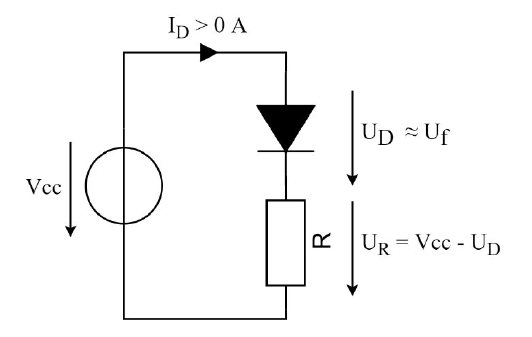
\includegraphics[width=0.3\textwidth]{Anhang/Schaltung1.png}
            \captionof{figure}{Schaltung der LED mit Taster}
            \figsource{\cite{bauer}}
            \label{fig:s1}
        \end{center}

    \paragraph{NAND-Schaltung}
        Be der NAND-Schaltung wurde der \texttt{SN74HC00N} verwendet. An zwei Eingängen wird je ein Taster mit einem hochohmigen Widerstand von \SI{10}{\kilo\ohm} als Pull-down geschalten. Die Verwendung der LED ist analog zur vorherigen Schaltung. Der Schaltplan ist in Abbildung \ref{fig:s2}.

        \begin{center}
            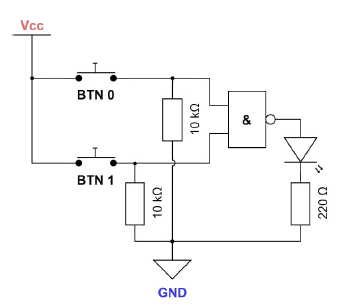
\includegraphics[width=0.5\textwidth]{Anhang/Schaltung2.png}
            \captionof{figure}{NAND-Schaltung}
            \figsource{\cite{bauer}}
            \label{fig:s2}
        \end{center}

    \paragraph{NOR-Schaltung}
        Der Schaltungsaufbau ist hier identisch zur NAND-Schaltung, lediglich der IC wird durch den \texttt{SN74HC02N} ausgetauscht. Abbildung \ref{fig:s3} zeigt den zugehörigen Schaltplan.

        \begin{center}
            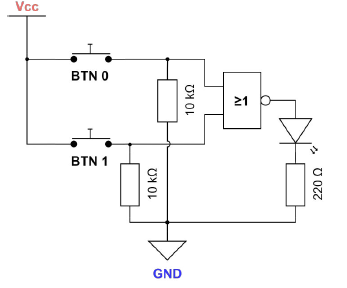
\includegraphics[width=0.5\textwidth]{Anhang/Schaltung3.png}
            \captionof{figure}{NOR-Schaltung}
            \figsource{\cite{bauer}}
            \label{fig:s3}
        \end{center}

    \paragraph{BCD-Codewandler}
        Erläuterungen zu den Eingängen LT, BI und LE sind dem Dokument "`Vorbereitung zum Versuch: Die digitale Zweifaltigkeit. Versuch 1"' von Jan Hoegen zu entnehmen. 
        
        Abbildung \ref{fig:s4} zeigt den Schaltungsaufbau.
        Die Kathoden der Anzeige werden an einen einzelnen \SI{1}{\kilo\ohm} Widerstand angeschlossen. Dies hat zur Folge, dass die Leuchtstärke der Anzeige bei verschiedenen Eingangszuständen nicht konstant ist. Am DIP-Schalter als Eingang werden erneut Pull-Down-Widerstände von \SI{10}{\kilo\ohm} verwendet.

        Statt des \texttt{M74C4511} wurde der \texttt{CD74HC4511E} verwendet. Die Funktion sowie die Belegung der Pins ist unverändert, das zugehörige Datenblatt \cite{datenblatt} befindet sich im Anhang \ref{app:2}.%
        % \footnote{Herausgeber: Texas Instruments. Abgerufen am 08.04.2022 von \url{https://www.ti.com/lit/ds/symlink/cd74hc4511.pdf?HQS=dis-mous-null-mousermode-dsf-pf-null-wwe&ts=1649347240369&ref_url=https\%253A\%252F\%252Fwww.mouser.com\%252F}}

        \begin{center}
            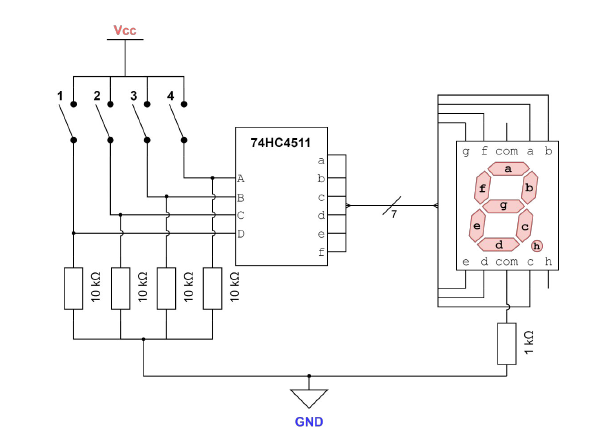
\includegraphics[width=0.5\textwidth]{Anhang/Schaltung4.png}
            \captionof{figure}{BCD-Codewandler}
            \figsource{\cite{bauer}}
            \label{fig:s4}
        \end{center}

\section{Aufbau}
    \label{sec:1}
    Zur Besseren Übersicht befinden sich die Fotoaufnahmen des Breadboardlayout im Anhang \ref{app:1} dieses Dokuments.

    Abbildung \ref{fig:1} zeigt den Aufbau der LED-Schaltung. Die NAND-Schaltung ist der Abbildung \ref{fig:2} zu entnehmen. Als nächstes wird der Aufbau der NOR-Schaltung in Abbildung \ref{fig:3} gezeigt. Zuletzt wird der BCD-Codewandler betrachtet. Der zugehörige Schaltungsaufbau wird in \ref{fig:4} gezeigt. 

\section{Analyse des Hardwareaufbaus}
    \paragraph{LED-Schaltung} Wenn der Taster geschlossen ist, leuchtet die LED auf. Dies entspricht den Erwartungen eines Schließers, da erst dann der Stromkreis geschlossen ist.

    \paragraph{NAND-Schaltung} Tabelle \ref{tab:1} zeigt den beobachteten Zusammenhang zwischen Taster und der LED der Schaltung. Erst dann, wenn beide Taster gleichzeitig betätigt werden, geht die LED aus. Dies entspricht den Erwartungen an ein NAND-Gatter.

    \begin{table}[H]
        \centering
        \caption{Wahrheitstabelle der NAND-Schaltung}
        \label{tab:1}
        \begin{tabular}{cc|c}\toprule
            T1  &   T2  &   LED\\\midrule
            0   &   0   &   1\\
            0   &   1   &   1\\
            1   &   0   &   1\\
            1   &   1   &   0\\\bottomrule
        \end{tabular}
    \end{table}

    \paragraph{NOR-Schaltung} Tabelle \ref{tab:2} zeigt den beobachteten Zusammenhang zwischen Taster und der LED der Schaltung. Die LED geht aus, sobald mindestens einer der beiden Taster betätigt werden. Dies entspricht den Erwartungen an ein NOR-Gatter.

    \begin{table}[h]
        \centering
        \caption{Wahrheitstabelle der NOR-Schaltung}
        \label{tab:2}
        \begin{tabular}{cc|c}\toprule
            T1  &   T2  &   LED\\\midrule
            0   &   0   &   1\\
            1   &   0   &   0\\
            0   &   1   &   0\\
            1   &   1   &   0\\\bottomrule
        \end{tabular}
    \end{table}

    \paragraph{BCD-Decoder} In der Tabelle \ref{tab:3} wird zu jeder Schalterstellung des DIP die angezeigte Ziffer notiert. Es fallen zwei Dinge auf: Zum einen entspricht die angezeigte Ziffer der Codierung im Datenblatt. Zum anderen sind alle Segmente aus, wenn ein Wert höher als \texttt{1001} eingestellt wird. Beides entspricht den Vorgaben im Datenblatt.
    
    \begin{table}[h]
        \centering
        \caption{Wahrheitstabelle des BCD-Codewandlers}
        \label{tab:3}
        \begin{tabular}{cccc|c}\toprule
            1   &   2   &   3   &   4   &   Ziffer\\\midrule
            0   &   0   &   0   &   0   &   0\\
            0   &   0   &   0   &   1   &   1\\
            0   &   0   &   1   &   0   &   2\\
            0   &   0   &   1   &   1   &   3\\
            0   &   1   &   0   &   0   &   4\\
            0   &   1   &   0   &   1   &   5\\
            0   &   1   &   1   &   0   &   6\\
            0   &   1   &   1   &   1   &   7\\
            1   &   0   &   0   &   0   &   8\\
            1   &   0   &   0   &   1   &   9\\\midrule
            1   &   0   &   1   &   0   &   \\
            1   &   0   &   1   &   1   &   \\
            1   &   1   &   0   &   0   &   \\
            1   &   1   &   0   &   1   &   \\
            1   &   1   &   1   &   0   &   \\
            1   &   1   &   1   &   1   &   \\\bottomrule
        \end{tabular}
    \end{table}

\section{Schlussfolgerungen}
    Es lässt sich folgern, dass Taster und IC so arbeiten, wie die Laboranleitung verlangt, und ein korrektes Schaltungsdesign verwendet wurde.   

    Der Taster arbeitet als Schließer und lässt einen Stromfluss zu, solange er gedrückt ist. Auch das NAND und das NOR arbeiten wie erwartet. Der BCD-Codewandler übersetzt einen Zustand am DIP-Schalter und die 7-Segment-Anzeige zeigt die dazugehörige Ziffer an. Für Eingangszustände größer als \texttt{1001} ist der Output als \textit{Blank} definiert. Daher bleibt in diesen Fällen das Display schwarz.

    Mir persönlich fiel es leicht, die Schaltungen aufzubauen und in Betrieb zu nehmen. Etwaige Fehler konnte ich schnell beheben. Auch die Tatsache, dass ich die Versuche nachgearbeitet habe, hat mich nur wenig beeinträchtigt.

\section{Verbesserungsvorschläge}

    % In diesem Versuchsbericht habe ich keine Schaltbilder oder andere Diagramme aus der Laboranleitung übernommen und hier erneut gezeigt. Ich bin mir nicht sicher, ob diese Vermeidung von Redundanz zu einem Nachteil für mich wird. Hätte der Bericht so formuliert werden sollen, dass auch ein außenstehender Leser die Ergebnisse nicht nur nachvollziehen, sondern auch nachbilden kann?

    Mir ist nicht klar, wie groß der Umfang des Kapitel \quoteenv{Schlussfolgerungen} sein soll. Jede Schaltung hat ihre Funktion erfüllt und es waren keine Abweichungen zu erkennen. Bis auf die Wahrheitstabellen mussten keine Messparameter beschrieben oder interpretiert werden.

\printbibliography[heading=bibintoc]

\appendix

\section{Anhang: Bilder der Schaltungen}
    \label{app:1}

    Abbildung \ref{fig:1} zeigt den Aufbau der LED-Schaltung. Die NAND-Schaltung ist der Abbildung \ref{fig:2} zu entnehmen. Als nächstes wird der Aufbau der NOR-Schaltung in Abbildung \ref{fig:3} gezeigt. Zuletzt wird der BCD-Codewandler betrachtet. Der zugehörige Schaltungsaufbau wird in \ref{fig:4} gezeigt.

    \begin{figure}[hb]
        \centering
        \begin{subfigure}[t]{0.5\textwidth}
            \centering
            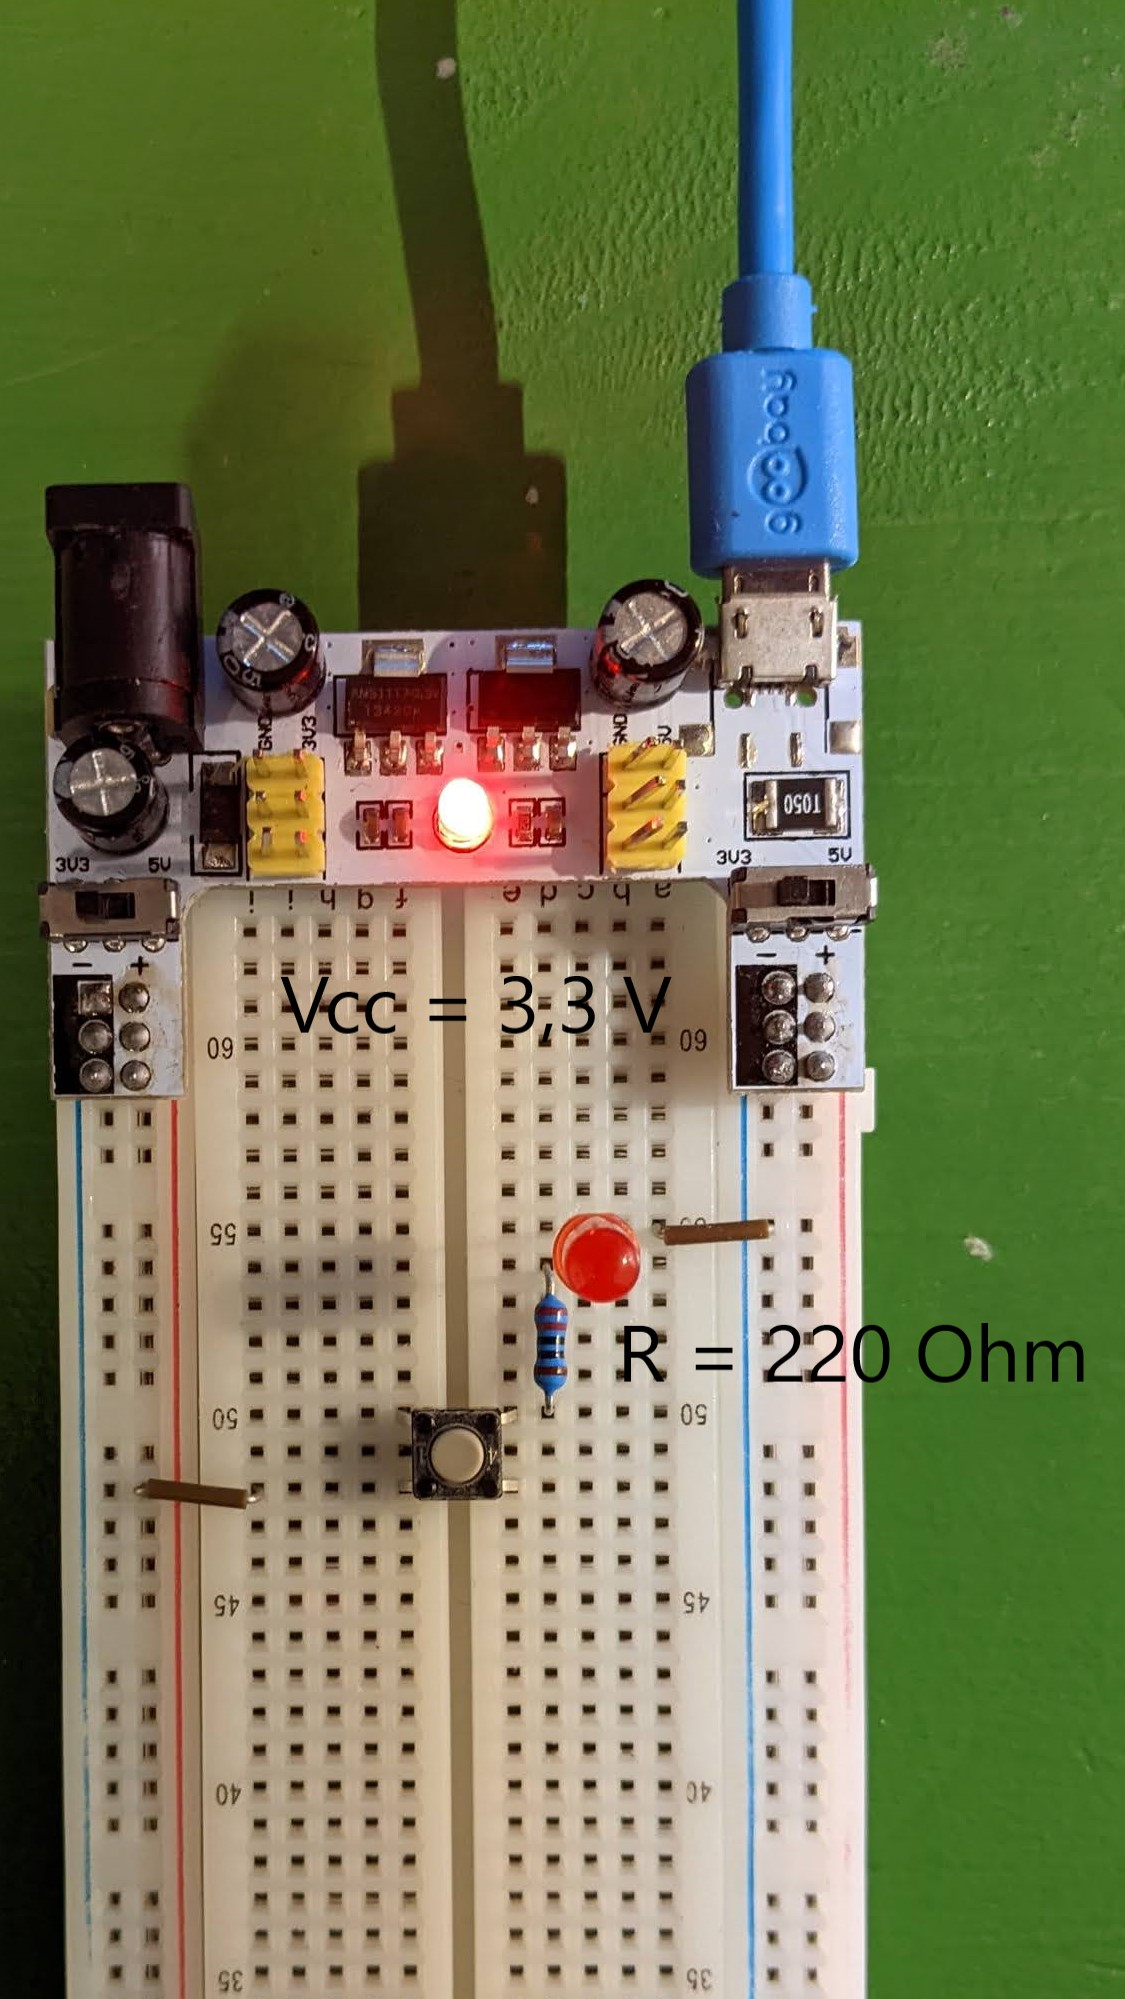
\includegraphics[width=0.5\linewidth]{Anhang/Bild1.1.jpg}
            \caption{Taster ist Offen}
        \end{subfigure}\hfill%
        \begin{subfigure}[t]{0.5\textwidth}
            \centering
            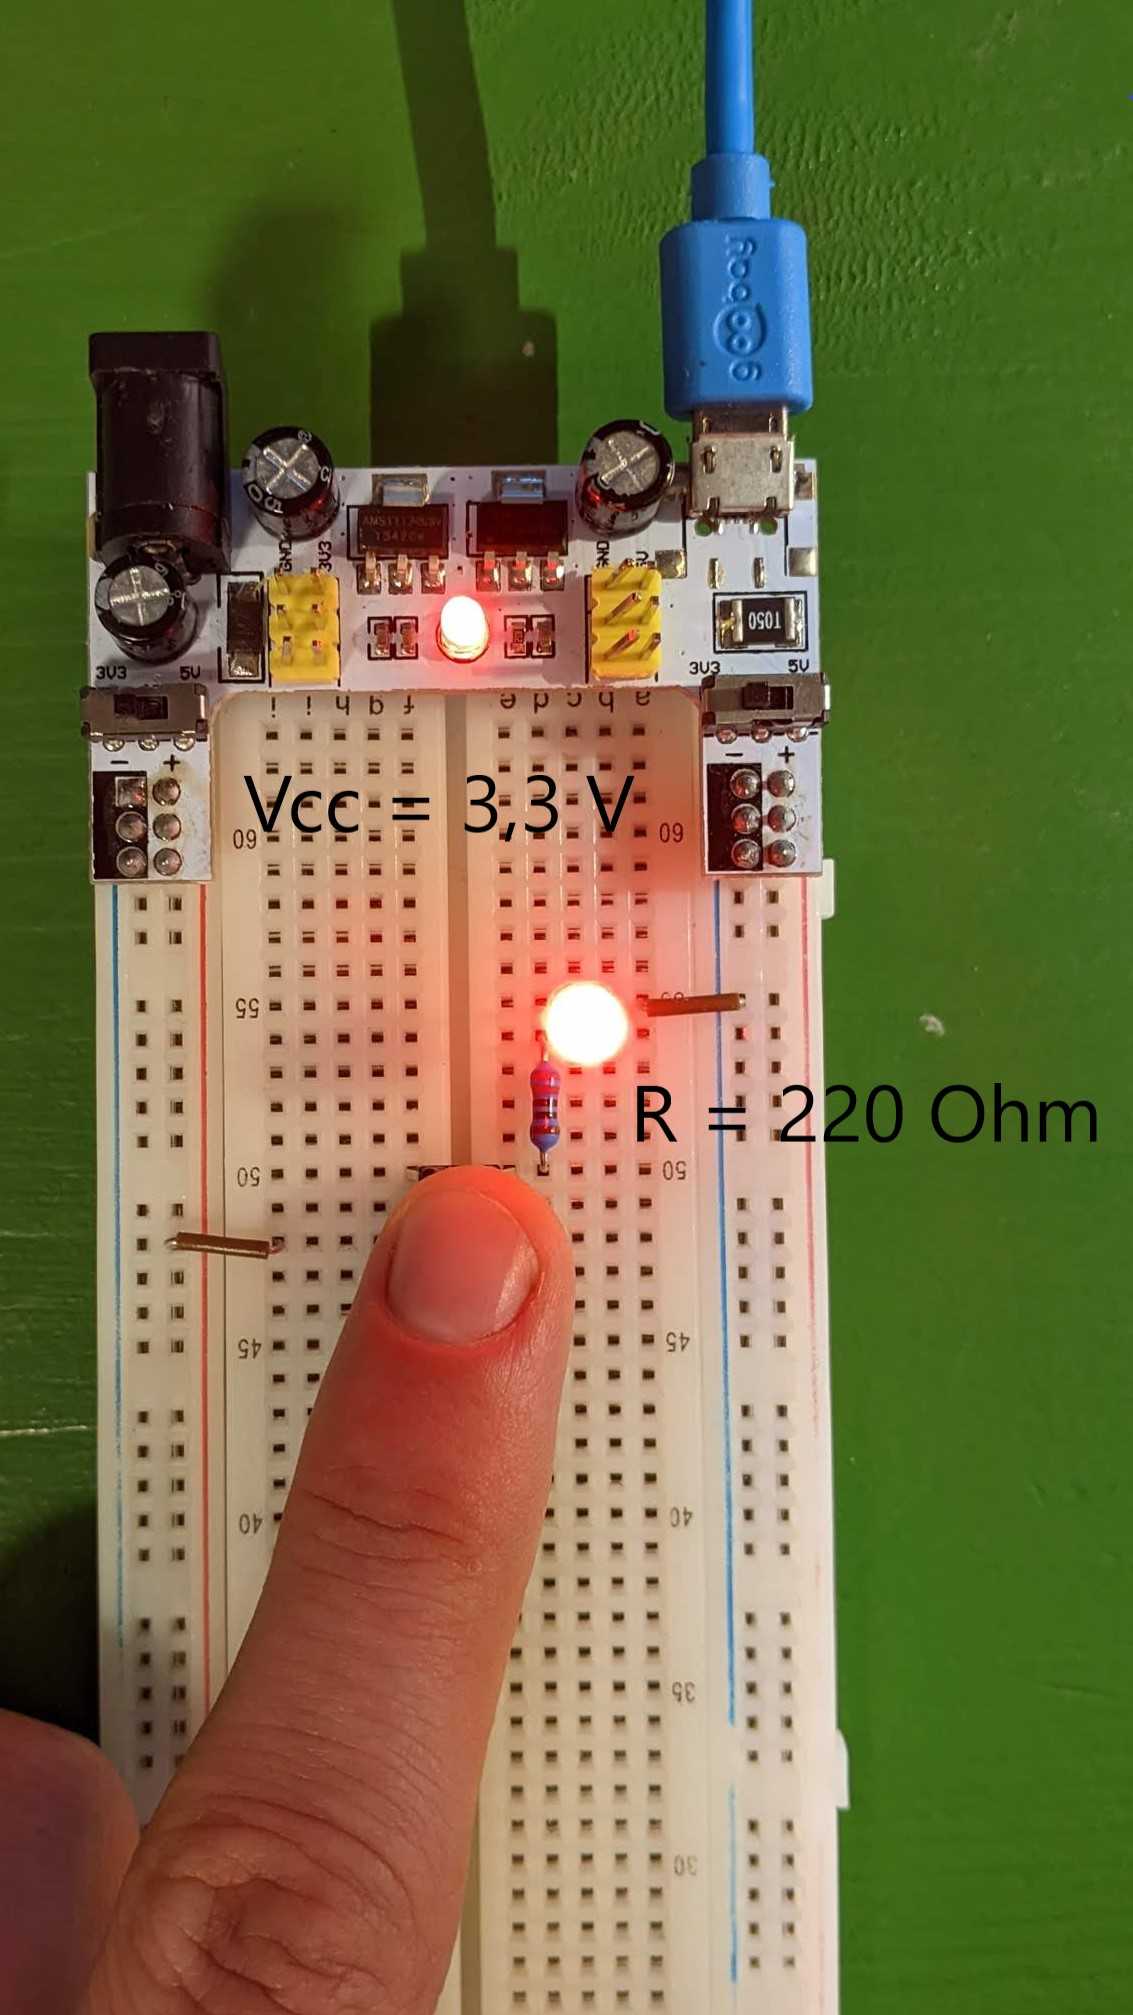
\includegraphics[width=0.5\linewidth]{Anhang/Bild1.2.jpg}
            \caption{Taster ist geschlossen}
        \end{subfigure}
        \caption{Realisierung der LED-Schaltung}
        \legend{\(R=\SI{220}{\ohm}, V_{cc}=\SI{3.3}{\volt}\)}
        \label{fig:1}
    \end{figure}

    \begin{figure}
        \centering
        \begin{subfigure}[t]{0.3\textwidth}
            \centering
            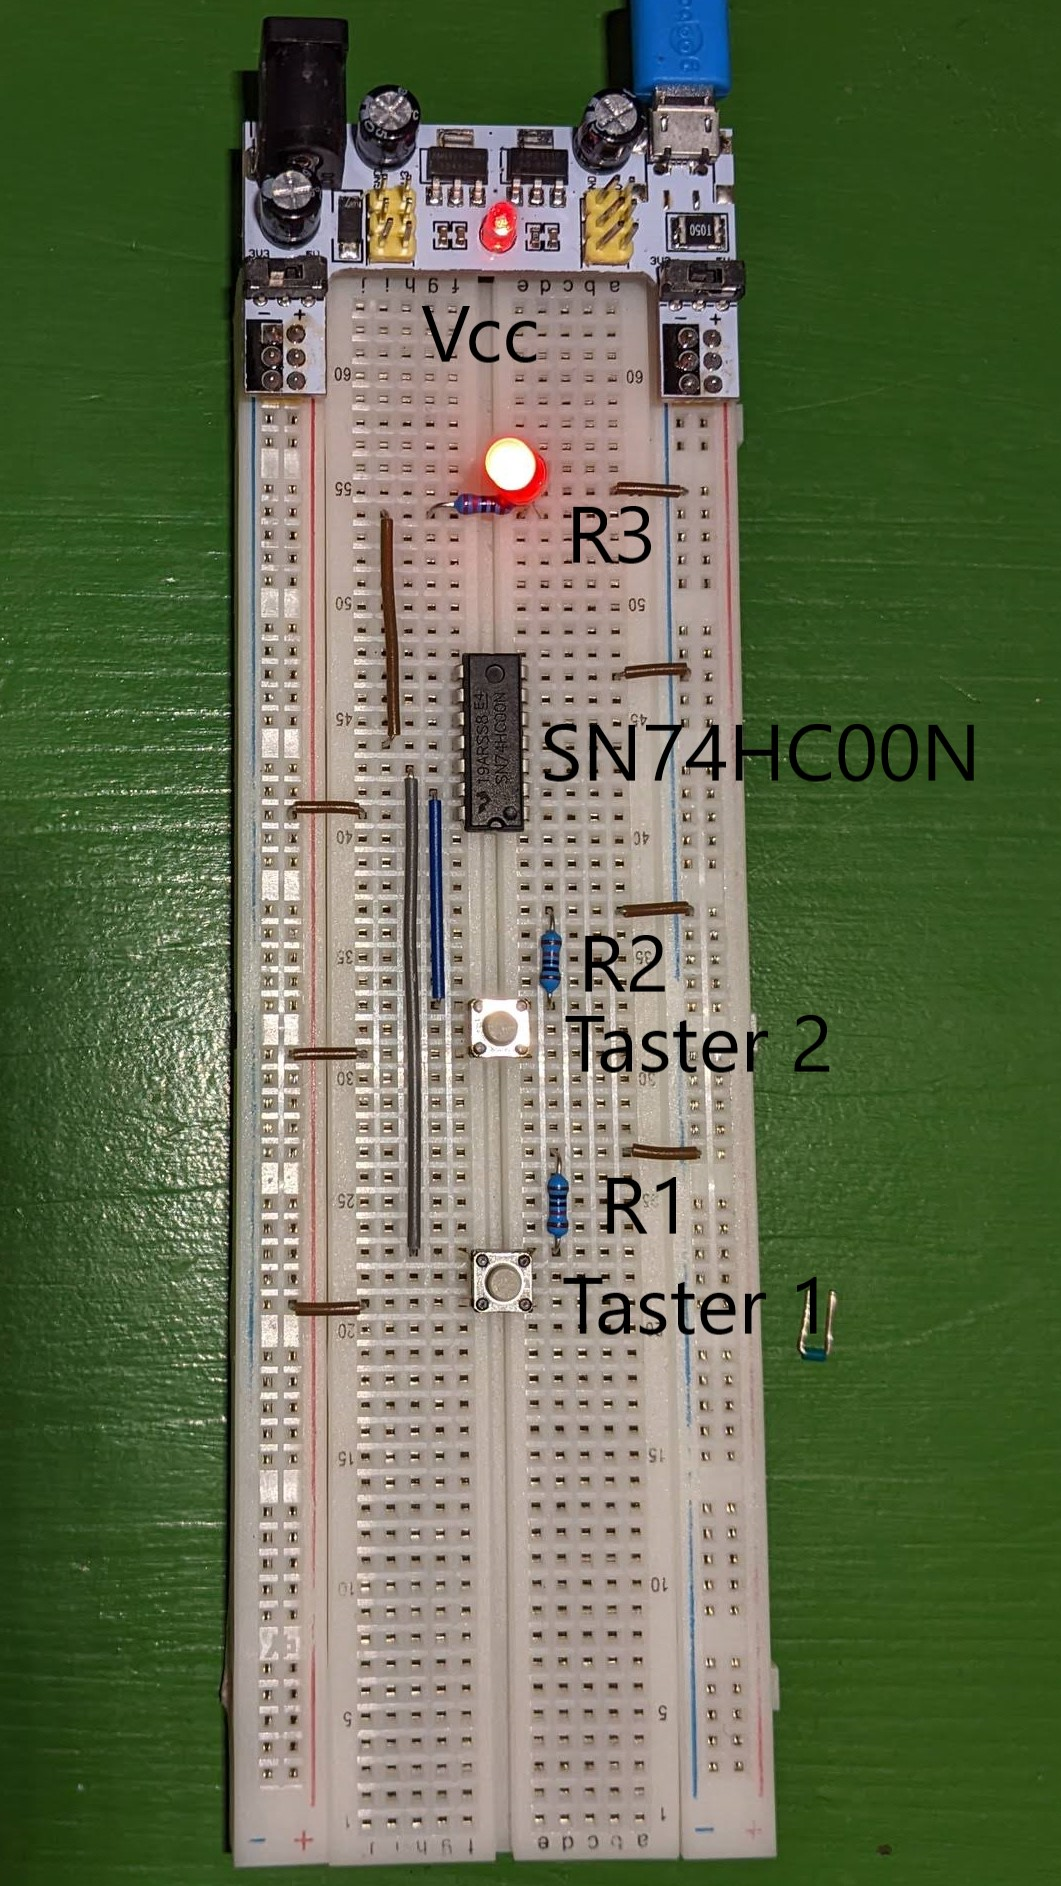
\includegraphics[width=0.9\linewidth]{Anhang/Bild2.1.jpg}
            \caption{Taster 1 und 2 sind offen}
        \end{subfigure}\hfill%
        \begin{subfigure}[t]{0.3\textwidth}
            \centering
            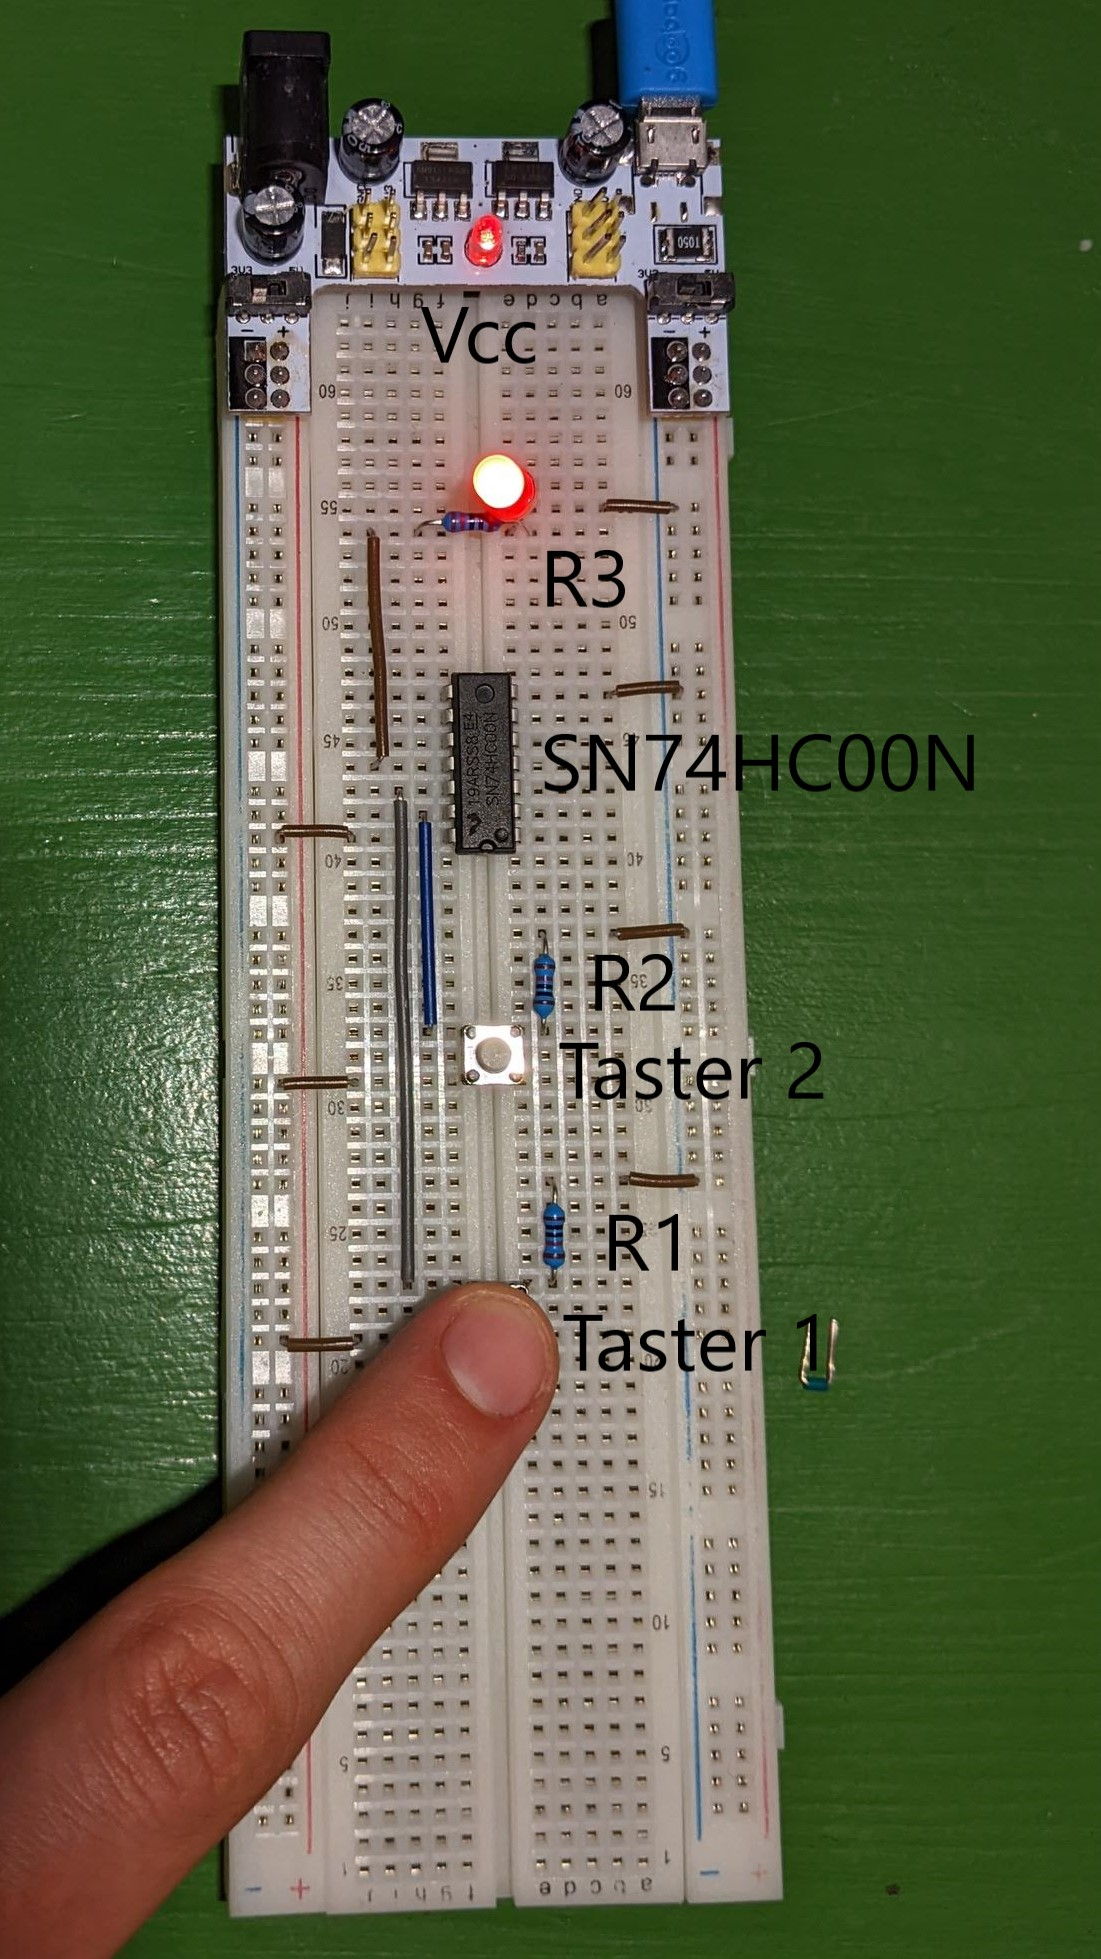
\includegraphics[width=0.9\linewidth]{Anhang/Bild2.2.jpg}
            \caption{Taster 1 ist geschlossen, Taster 2 ist offen}
        \end{subfigure}\hfill%
        \begin{subfigure}[t]{0.3\textwidth}
            \centering
            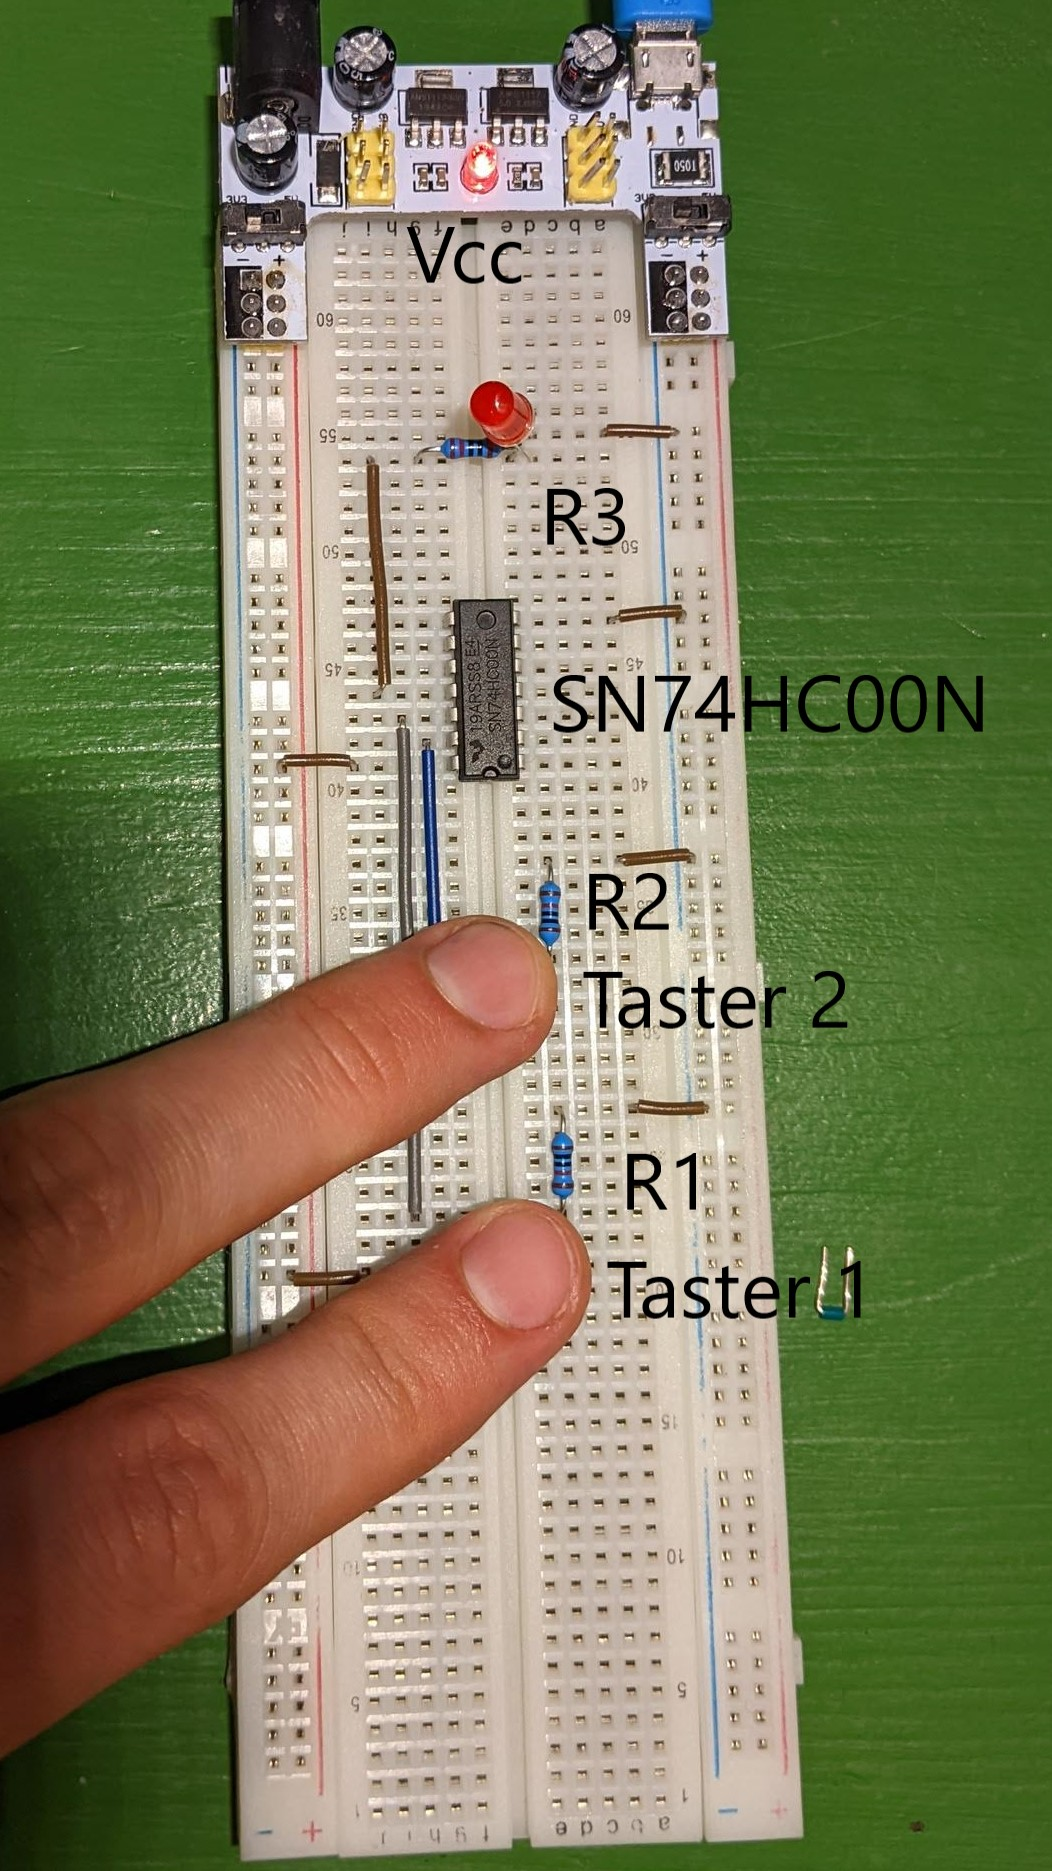
\includegraphics[width=0.9\linewidth]{Anhang/Bild2.3.jpg}
            \caption{Taster 1 und 2 sind geschlossen}
        \end{subfigure}
        \caption{Realisierung der NAND-Schaltung}
        \legend{\(R_1=R_2=\SI{10}{\kilo\ohm}, R_3=\SI{220}{\ohm}, V_{cc}=\SI{3.3}{\volt}\)}
        \label{fig:2}
    \end{figure}

    \begin{figure}
        \centering
        \begin{subfigure}[t]{0.3\textwidth}
            \centering
            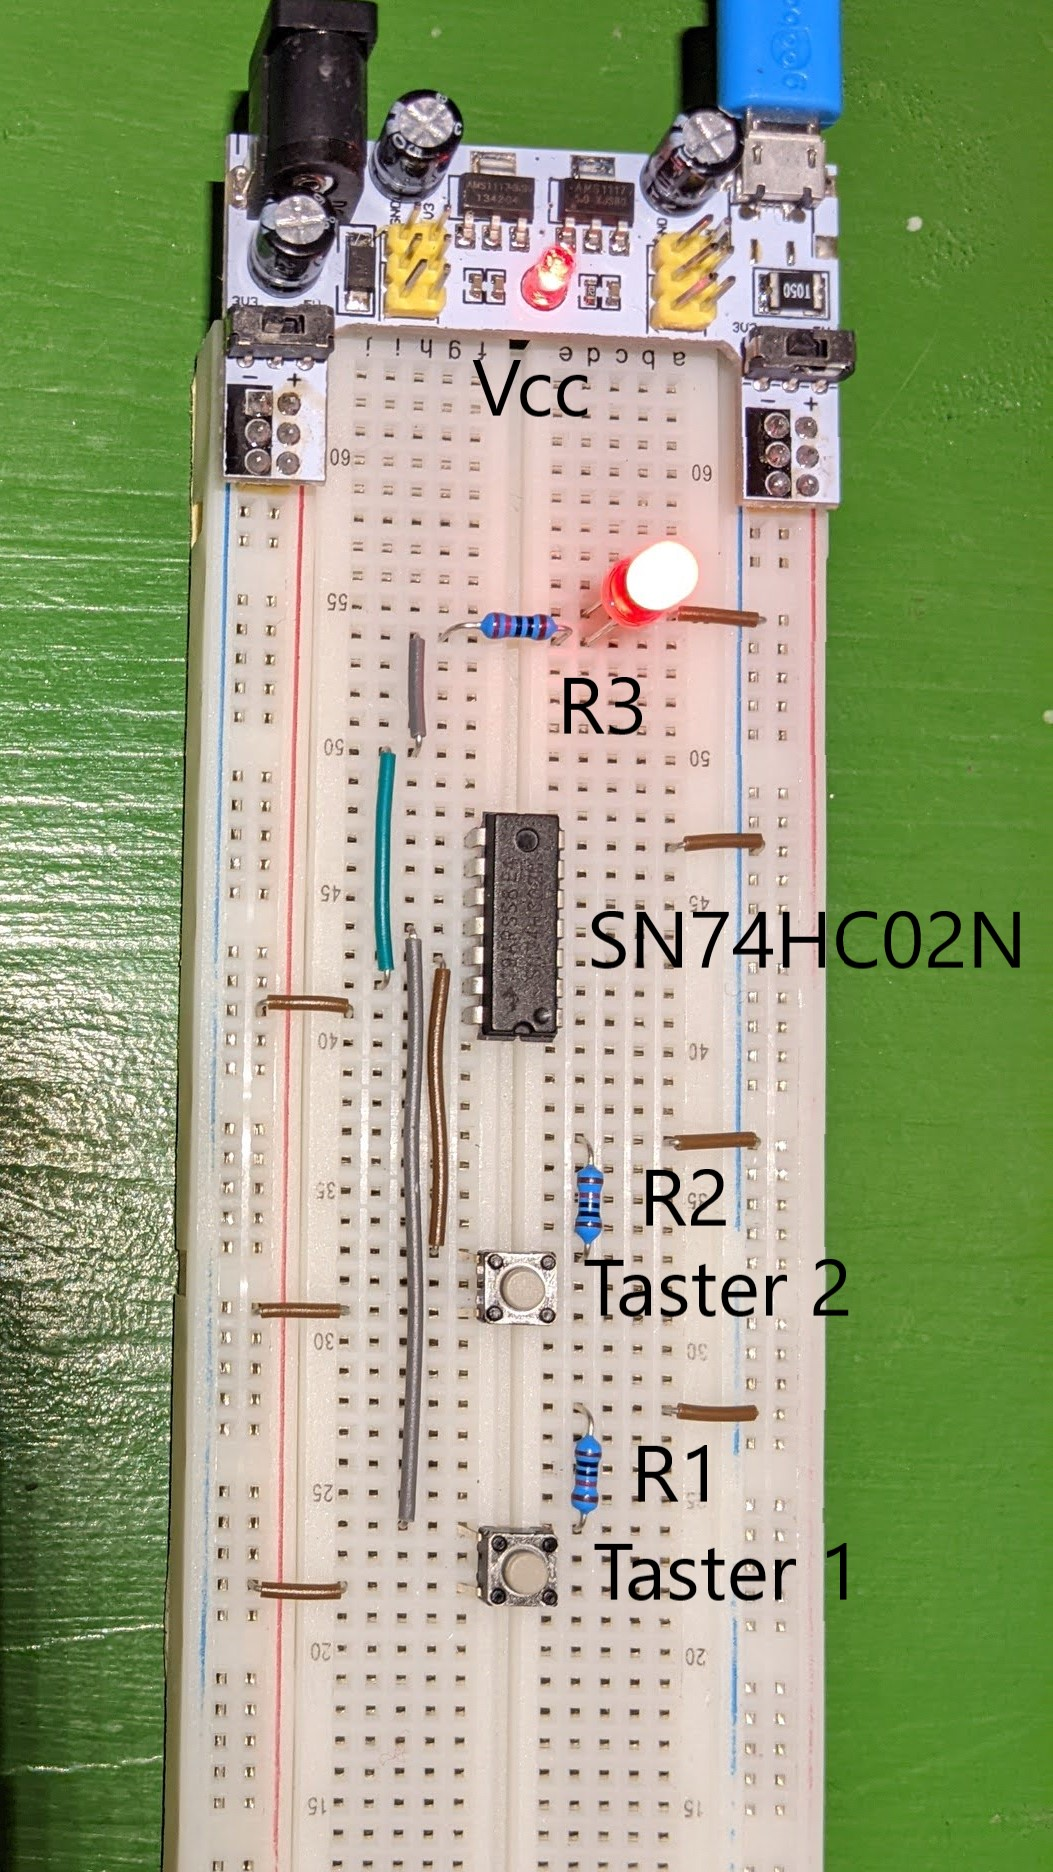
\includegraphics[width=0.9\linewidth]{Anhang/Bild3.1.jpg}
            \caption{Taster 1 und 2 sind offen}
        \end{subfigure}\hfill%
        \begin{subfigure}[t]{0.3\textwidth}
            \centering
            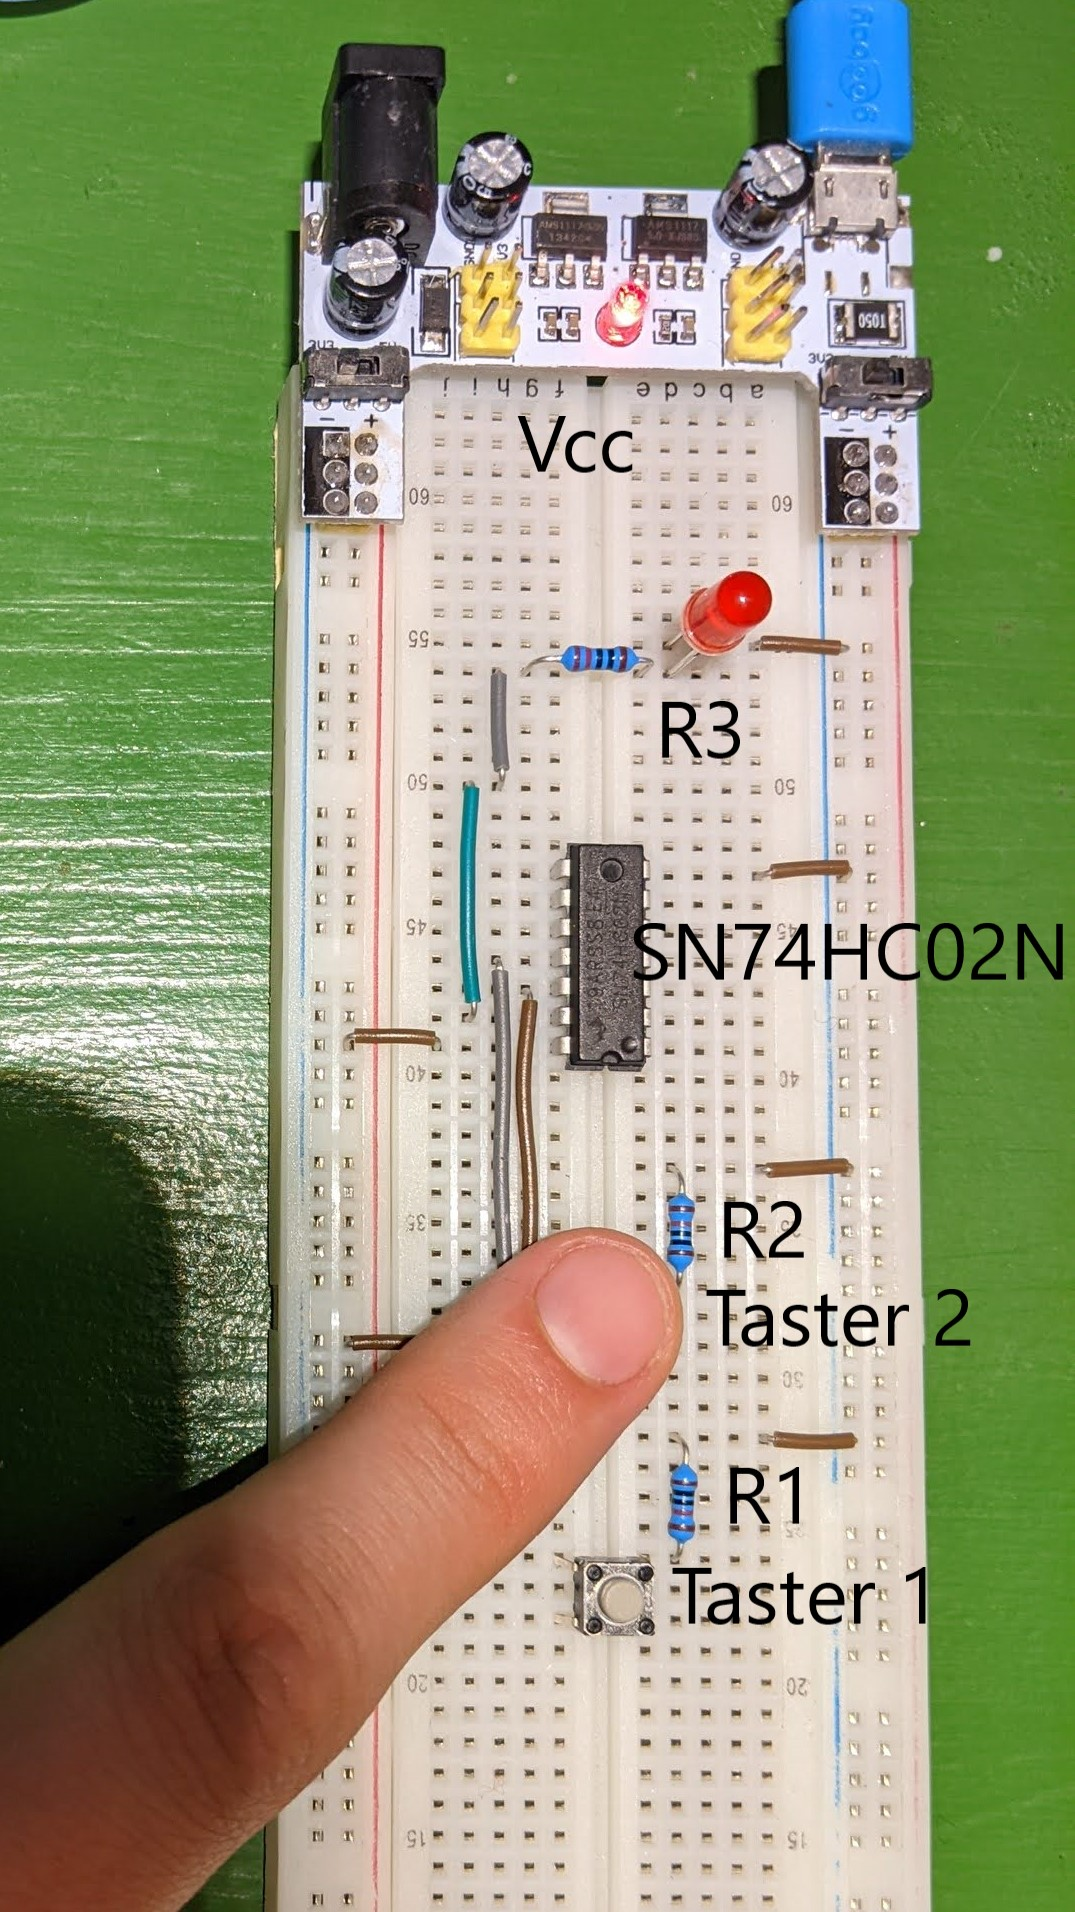
\includegraphics[width=0.9\linewidth]{Anhang/Bild3.2.jpg}
            \caption{Taster 1 ist offen, Taster 2 ist geschlossen}
        \end{subfigure}\hfill%
        \begin{subfigure}[t]{0.3\textwidth}
            \centering
            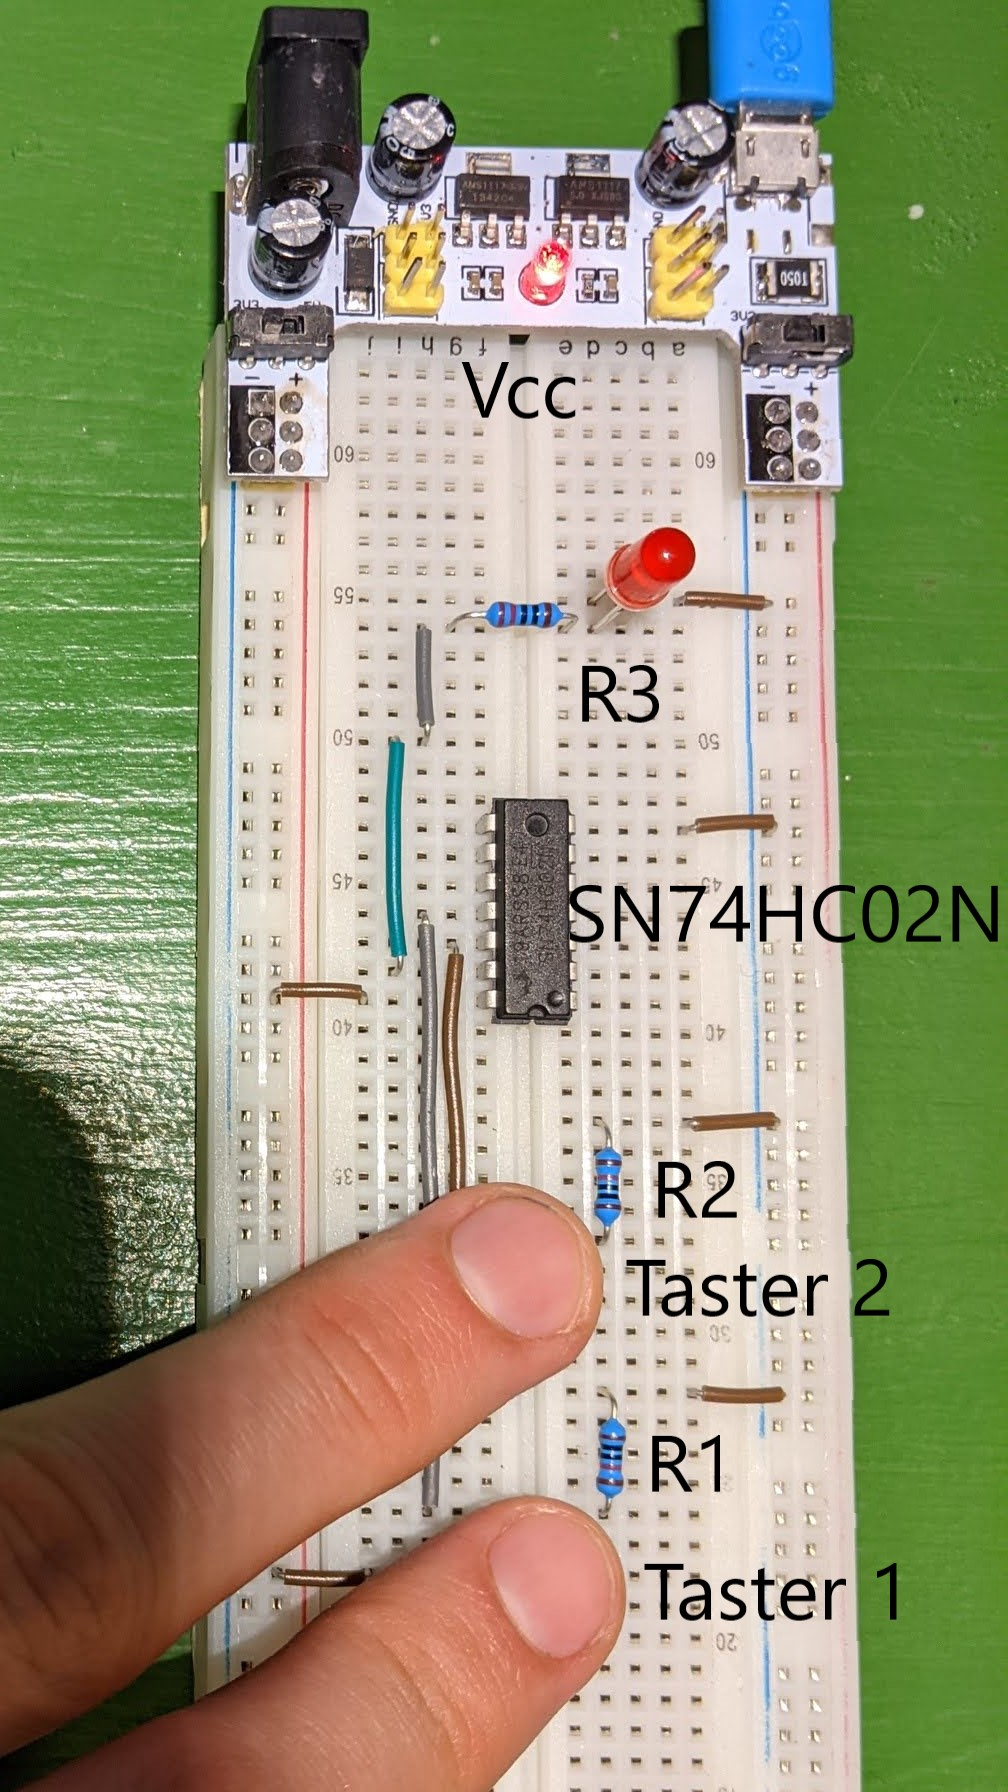
\includegraphics[width=0.9\linewidth]{Anhang/Bild3.3.jpg}
            \caption{Taster 1 und 2 sind geschlossen}
        \end{subfigure}
        \caption{Realisierung der NOR-Schaltung}
        \legend{\(R_1=R_2=\SI{10}{\kilo\ohm}, R_3=\SI{220}{\ohm}, V_{cc}=\SI{3.3}{\volt}\)}
        \label{fig:3}
    \end{figure}

    \begin{figure}
        \centering
        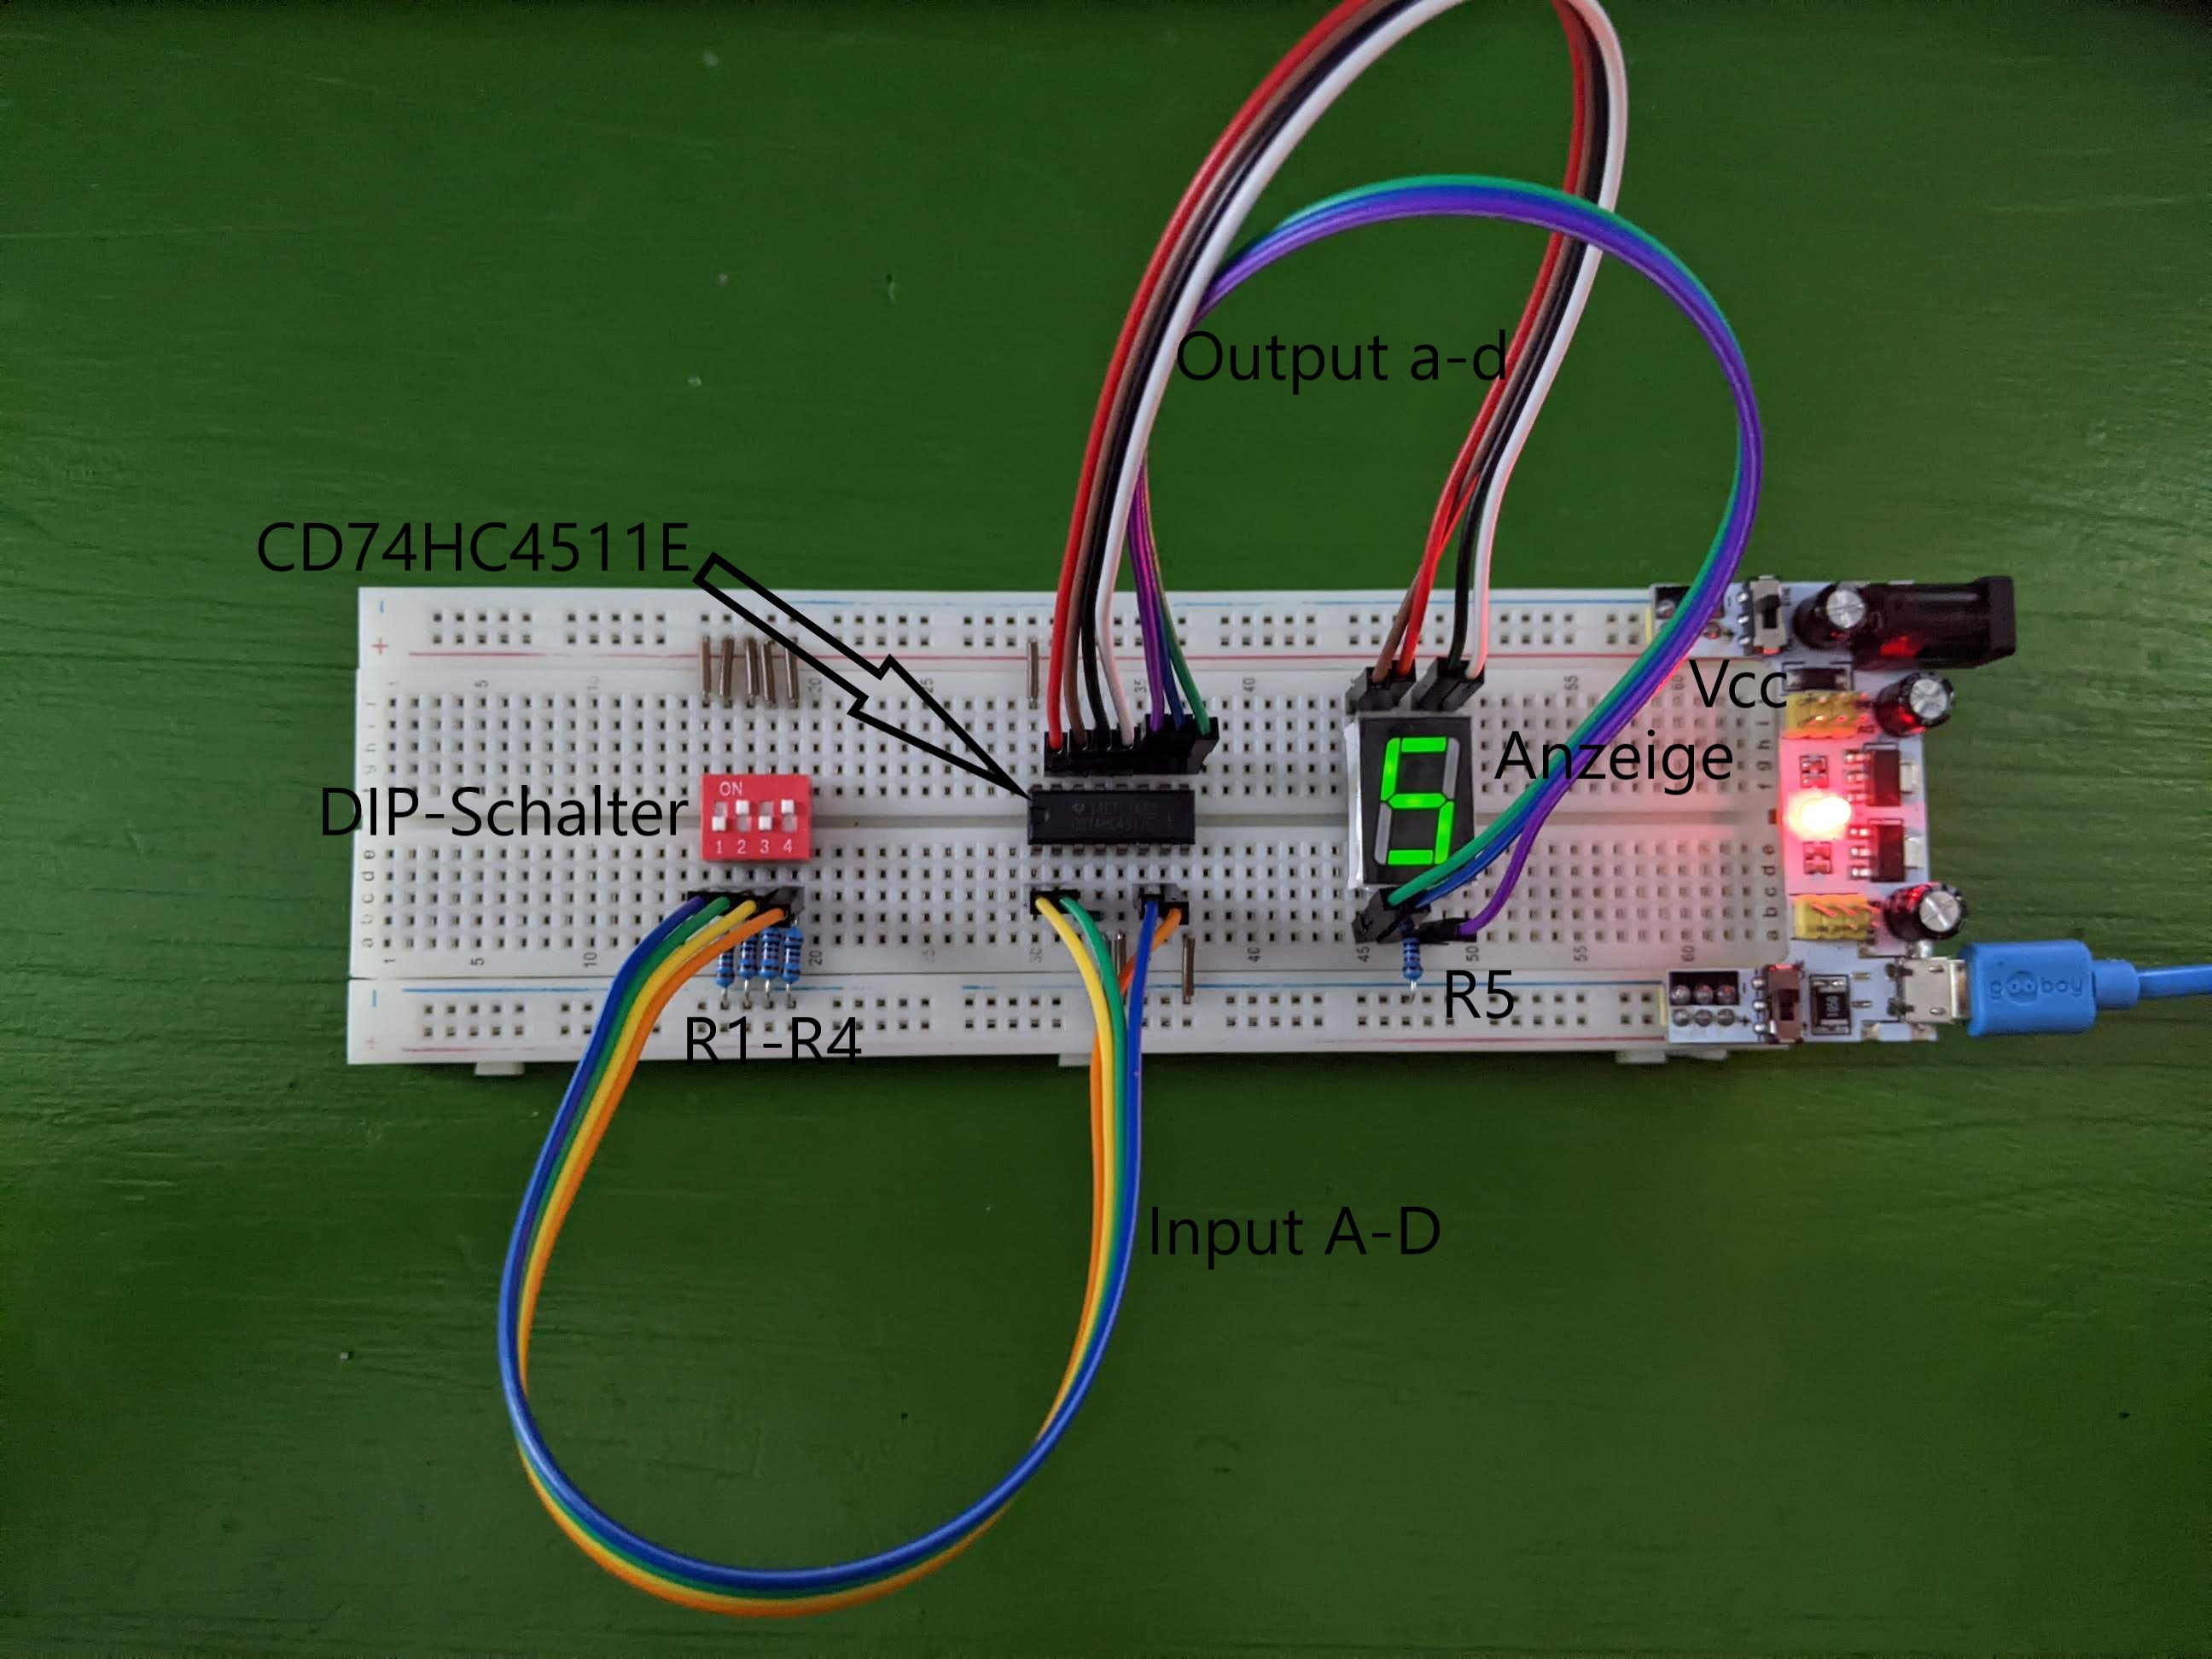
\includegraphics[width=0.7\textwidth]{Anhang/Bild4.jpg}
        \caption{Realisierung des BCD-Decoder}
        \legend{\(R_1=R_2=R_3=R_4=\SI{10}{\kilo\ohm}, R_5=\SI{1}{\kilo\ohm}, V_{cc}=\SI{3.3}{\volt}\)}
        \label{fig:4}
    \end{figure}

\clearpage

\shadowsection{Anhang: Datenblatt des BCD-Codewandlers}
    \label{app:2}
    
\includepdf[pages=-]{Anhang/Datenblatt.pdf}

\end{document}